\subsection{Setup}\label{setup}
This chapter explains features, which were not implemented as the project was started. This features are mainly to grow the community, as offering features to make starting coding with Dafny easier and support a wide range of IDEs. The goal of the explain why they were chosen and implemented. 
\subsubsection{Language Server} \label{setupLanguageServer}
\paragraph{What is a Language Server}
A language server allows to integrate features like auto completion, go to definition, find all references in an easy way into IDEs. Such a server mostly coexists with a client, which is a normally a native IDE plugin, which does the customization of the GUI, register shortcuts or adds menu items. The language server provides a list of supported actions, which are normally shown in the IDE. This makes it very handy to extend it as well. 
The protocol between these two components is standardized by Microsoft, with the idea behind, make it IDE independent. 
 \newline
\begin{figure}[H]
	\centering
	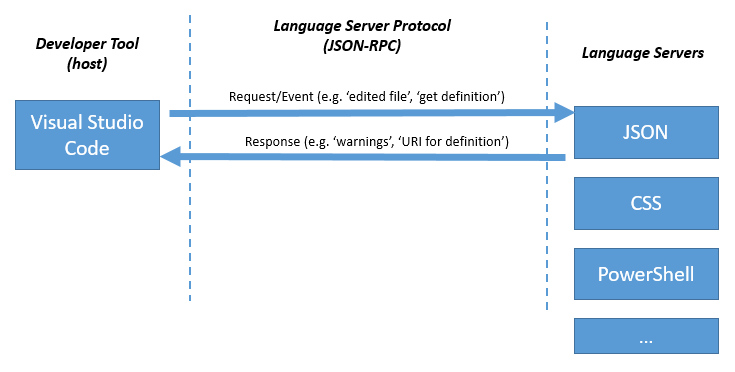
\includegraphics[width=1.0\textwidth]{img/languageServer}
	\caption{Language Server}
	\label{fig:languageServer}
\end{figure}
\paragraph{Why were they chosen to implement}
Since Dafny is already supported on different operation systems, it was decided to make the plugin as platform and IDE independent as possible. Because Visual Studio Code supports the Language Server Protocol and is the reference implementation, the existing plugin was refactored to work as a language server. The strictly split of the plugin into a client and a server had also the benefit, that the architecture had to be changed, which resulted in a much better and clearer structure. \newline
In the future another IDE could just integrate the existing language server, make smaller tweaks to the client and it would work. No rewriting of the whole logic, just use the server and most features will just work, thanks to the standardized protocol. 
\paragraph{What benefits do they entail}
Developing the plugin as a language server has the big benefit, that it could be easily integrated into existing IDEs, which supports Language Server Protocol, without reprogramming everything. Supporting auto completion, go to definition, find all references, would just work, without writing a single line of code. The only step is to start the Language Server and connect to it. Only the client is needed to be adjusted, depending on the requirements how the GUI should look like and mostly the programming language to developing the client will change. 
See \ref{ides} for a overview of IDEs which were looked at and tried to be supported. 
\subsubsection{Automatic Installation} \label{setupAutomaticInstallation}
\paragraph{What is Automatic Installation}
Automatic Installation is the process to setup the whole Dafny environment in the background. Downloading the latest release from GitHub, extract it and setting all necessary configuration properties correctly. This process is platform dependent, because there is a zip for each operating system. 
\paragraph{Why was this chosen to implement}
The setup to start coding with Dafny was quite complicated. The whole installation was not straightforward. First download the Dafny.zip from GitHub, which is hidden under releases. Second extract it to a directory. Afterwards install the Dafny plugin for Visual Studio Code, set the path to the DafnyServer.exe. You never knew exactly if it was the path with or without DafnyServer.exe. Finally after a restart of Visual Studio Code it maybe worked. \newline
Because this is quite complicated, especially if you want the grow the community, this process must be much easier. For this reason it was decided to implement this important feature. The goal was that a new user can start coding in under 1 minute. 
\paragraph{What benefits do this entail}
More people can start writing Dafny programs, not worrying setting up Dafny, struggling in configurations or do not find the release on GitHub. Also professors can integrate Dafny into their lectures, as long as students can install Dafny without problems. 
\subsubsection{Automatic Upgrade} \label{setupAutomaticUpgrade}
\paragraph{What is Automatic Upgrade}
Automatic Upgrade makes sure, that always the latest version of Dafny is used. If a new release is published on GitHub this feature will check that, and notify the user, that there is newer release available. If the user wants to upgrade the Dafny environment, the feature \ref{setupAutomaticInstallation} will take over. 
\paragraph{Why was this chosen to implement}
Most people will never look at GitHub to check if there is a newer version of Dafny available. Especially if there is no need to, because everything can be installed automatically. Out of this reason, there need a version check, which informs the user if there is a newer version. 
\paragraph{What benefits do this entail}
Newer versions bring important bug fixes and new features, which would not be used if there is no version check. Users can install newer version the same easy way, as installing the environment the first time.  
